% =====================================================================
% פרק 6 — עמידות המערכת מול ״קיר המסירות״ 2026–2027 ובחינת ההשערות
% RESEARCH_CORE_AGENT (Agent 2)
% =====================================================================
\chapter{עמידות המערכת מול ״קיר המסירות״}
\label{ch:delivery-wall}

\begin{managerbox}
ביום המסירה הרוכש צריך לקבל משכנתא, היזם צריך לגבות את יתרת התמורה כדי לפרוע את אשראי הליווי, והבנק צריך שהבטוחה תכסה את חשיפתו, כולל ערבויות חוק המכר. הפרק מאתר את ספי הכשל ומכריע בהשערות. למעקב: הריבית, המחירים והעיכובים.
\end{managerbox}

\section{צד הרוכשים: יחס ההחזר ביום המסירה}
\label{sec:ch6-buyers}\label{sec:ch6-facts}

רוכש שחוצה את תקרת ה־\pct{50} של הוראה \en{329} (סעיף~\ref{sec:ch3-baseline}) לא יקבל את מלוא המשכנתא, ויצטרך להשלים הון, למכור את הזכות או לבטל (סימולציה: איור~\ref{fig:pti-mc}). התוצאות הן תרחיש, לא תחזית (סעיף~\ref{sec:ch5-limitations}).

\begin{figure}[!htb]
\centering
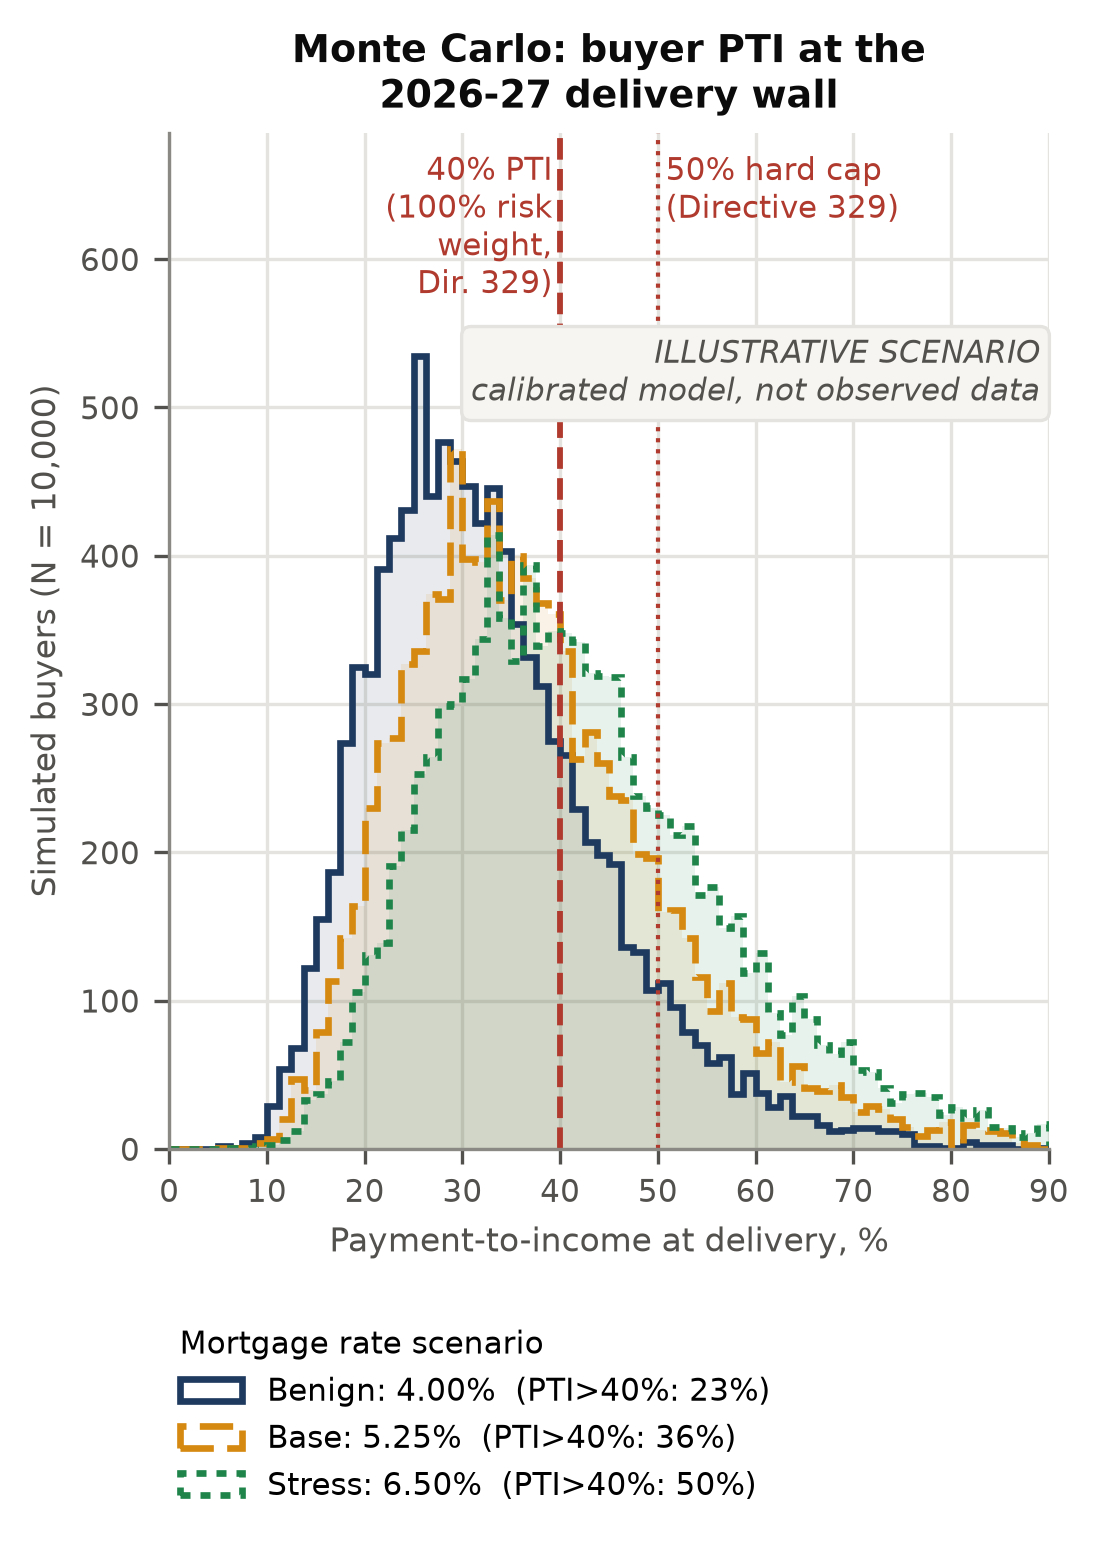
\includegraphics[width=0.62\textwidth]{figures/fig4_pti_monte_carlo.png}
\caption[יחס ההחזר ביום המסירה בשלושה תרחישי ריבית (תרחיש)]{התפלגות יחס ההחזר מההכנסה ביום המסירה (מונטה קרלו, \en{N=10,000}; תרחיש להמחשה)}
\label{fig:pti-mc}
\end{figure}

\label{tab:ch6-pti}בריביות \pct{4.00}, \pct{5.25} ו־\pct{6.50}, בהתאמה, החציון הוא \pct{30.9}, \pct{35.4} ו־\pct{40.2} (אחוזון \en{90}: \pct{48.2}, \pct{55.3} ו־\pct{62.7}); \pct{23.1}, \pct{36.1} ו־\pct{50.5} מהרוכשים חוצים את \pct{40}, ו־\pct{8.4}, \pct{16.0} ו־\pct{26.7} חוצים את \pct{50}. הריבית היא אפוא המשתנה הדומיננטי. סייגים: חציון המחיר וההכנסה הם הנחות, והרוכש אינו יכול להגדיל הון עצמי במודל.


\section{צד היזמים והבנקים: רשת מבחני הקיצון}
\label{sec:ch6-developers}

איור~\ref{fig:stress-grid} מציג את \term{יחס כיסוי שירות החוב}{DSCR} של היזם (משוואה~\ref{eq:ch5-dscr}) ואת כיסוי הבטוחות של הבנק (משוואה~\ref{eq:ch5-coverage}) בפרויקט המייצג.

\begin{figure}[!htb]
\centering
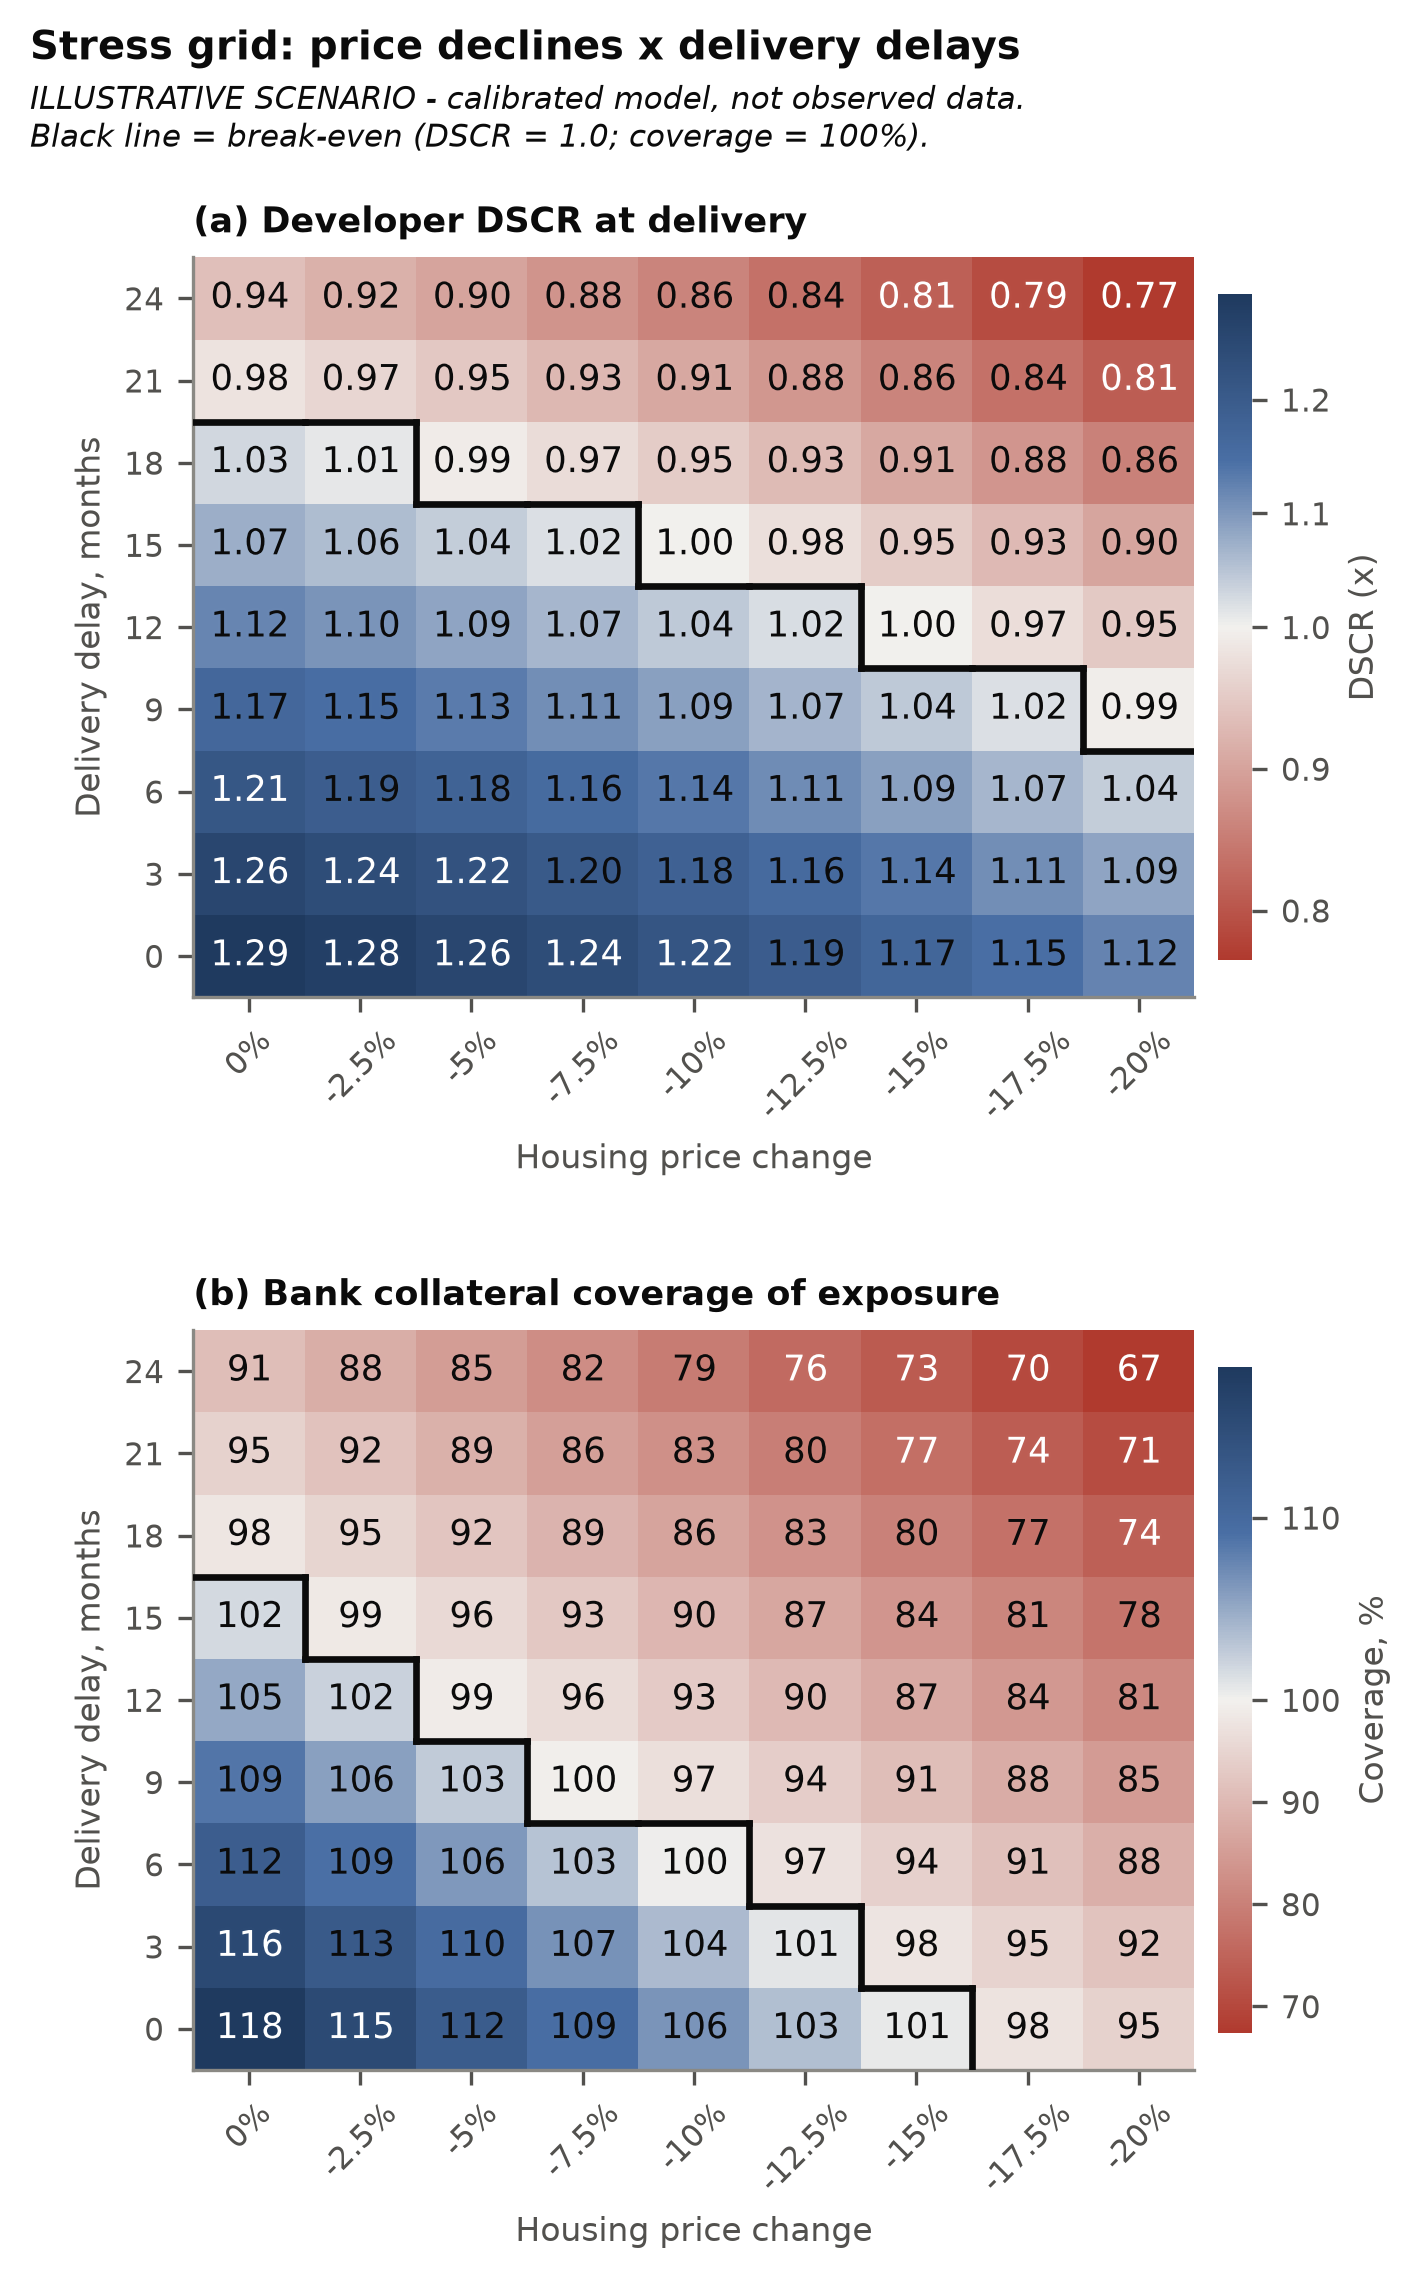
\includegraphics[width=0.85\textwidth]{figures/fig5_delivery_wall_resilience_heatmap.png}
\caption[רשת מבחני קיצון: \en{DSCR} וכיסוי הבטוחות (תרחיש)]{רשת מבחני קיצון לפרויקט מייצג: (\en{a}) \en{DSCR} של היזם; (\en{b}) כיסוי הבטוחות של הבנק כאחוז מחשיפתו. הקו השחור מסמן את נקודת האיזון. תרחיש מכויל להמחשה}
\label{fig:stress-grid}
\end{figure}

\textbf{היזם.} בתרחיש הבסיס ה־\en{DSCR} הוא \en{1.29}, ובתרחיש החמור ביותר ברשת (\pct{-20}, \en{24} חודשים) \en{0.77}. ב־\en{34} מתוך \en{81} תאים הוא נמוך מ־\en{1}; כבר בלחץ מתון (\pct{-10}, \en{12} חודשים) הוא רק \en{1.04}.

\textbf{הבנק.} הכיסוי יורד מ־\pct{118} בבסיס ל־\pct{67} בתרחיש החמור, וב־\en{57} מתוך \en{81} תאים הוא נמוך מ־\pct{100}. כשהיזם נכשל, ערבויות חוק המכר מגדילות את חשיפת הבנק כשהבטוחה נשחקת.

\textbf{רגישות.} עיכוב של שלושה חודשים שקול בקירוב לירידת מחירים של \pct{5} עבור ה־\en{DSCR} של היזם, ולירידה של \en{2.5\%–3\%} עבור כיסוי הבטוחות של הבנק.

\section{צד הבנקים: שחיקת ההון העצמי}
\label{sec:ch6-cet1}

לפי מודל שחיקת ההון (סעיף~\ref{subsec:ch5-cet1}), בתרחיש החמור שנקבע מראש (כשל רוכשים של \pct{25}, ירידת מחירים של \pct{20} ועיכוב של \en{24} חודשים) ההפסד לפני מס הוא \nis{48.0} מיליארד, \pct{21.3} מההון העצמי של המערכת, בגרסה $A$ השמרנית, ו־\nis{31.9} מיליארד, \pct{14.2}, בגרסה $B$ המבנית (אחרי מס: \pct{13.9} ו־\pct{9.2}). יחס \term{ההון העצמי רובד \en{1}}{CET1} המערכתי יורד מ־\pct{10.96} ל־\pct{9.44} ($A$, \en{152} נ״ב) או ל־\pct{9.96} ($B$, \en{101} נ״ב; איור~\ref{fig:cet1-erosion}).

\begin{figure}[!htb]
\centering
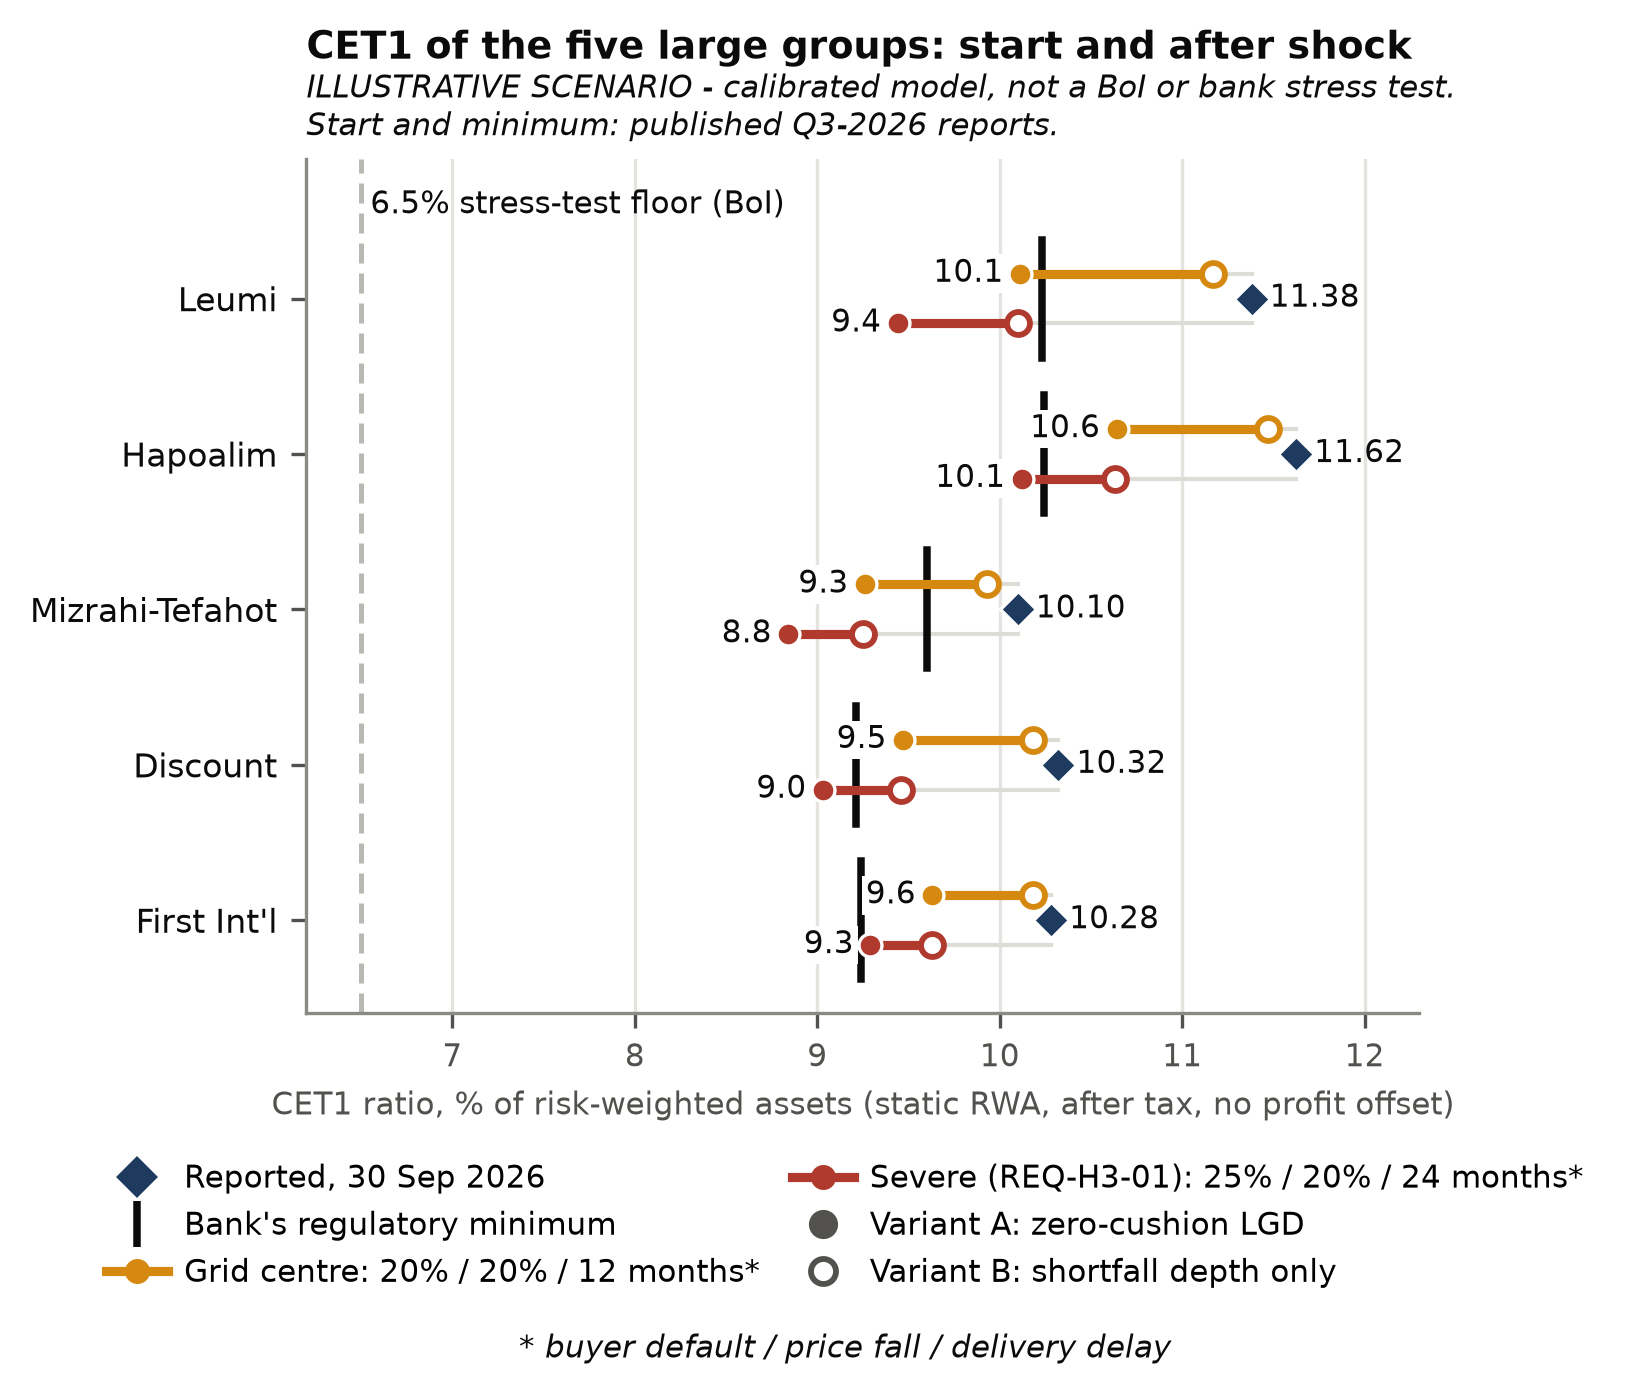
\includegraphics[width=0.85\textwidth]{figures/fig7_bank_cet1_erosion.png}
\caption[יחס \en{CET1} של הבנקים לפני הזעזוע ואחריו (תרחיש)]{יחס \en{CET1} לפני הזעזוע ואחריו מול המזערי (מלא: $A$; ריק: $B$; תרחיש, לא מבחן רשמי)}
\label{fig:cet1-erosion}
\end{figure}

\textbf{היחס המזערי (להמחשה).} בגרסה $A$ ארבע קבוצות יורדות אל מתחת ליחס המזערי (טבלה~\ref{tab:ch5-banks}): לאומי (\pct{9.44}), הפועלים (\pct{10.12}), מזרחי־טפחות (\pct{8.84}) ודיסקונט (\pct{9.03}); הבינלאומי נותר מעליו (\pct{9.29}). בגרסה $B$ רק לאומי (\pct{10.10}) ומזרחי־טפחות (\pct{9.25}). חריגה מיחס מזערי אינה חדלות פירעון: באף אחד מהתרחישים שנבחנו בפרמטרי הבסיס (עד כשל \pct{40}, ירידה \pct{40} ו־\en{24} חודשים) אין בנק היורד אל מתחת ל־\pct{6.5}, רצפת מבחני הקיצון \cite{boi_survey2024}; בגרסה $A$ (כשל \pct{25}, \en{24} חודשים) היא נחצית לראשונה בירידה של \pct{41.2}.

\textbf{עמידות הממצא.} כל \en{25} התאים בעיכוב של \en{24} חודשים חורגים מ־\pct{10} בשתי הגרסאות (טבלה~\ref{tab:ch6-grid}; שורות: כשל $\delta$, עמודות: ירידה $q$). ב־\en{12} חודשים טווח ההפסד הוא \en{7.5\%–19.9\%} ($A$) ו־\en{0.5\%–4.8\%} ($B$), ובמרכז הרשת \pct{14.0} ו־\pct{2.4}; ללא עיכוב הוא לכל היותר \pct{1.3} ($A$) ואפס ($B$). כשל רוכשים לבדו אינו יוצר הפסד בנקאי.

\begin{table}[!htb]
\centering
\caption[רשת \en{5×5}: הפסד בנקאי ב־\en{24} חודשים (תרחיש)]{הפסד בנקאי ב־\en{24} חודשים, אחוז מההון לפני מס (\en{A / B}; תרחיש; מודגש: ההכרעה)}
\label{tab:ch6-grid}
\footnotesize
\begin{tabularx}{\tabmaxwidth}{>{\centering\arraybackslash}p{1.9cm} C C C C C}
\toprule
\hd{$\delta$ / $q$} & \hd{\pct{15}} & \hd{\pct{17.5}} & \hd{\pct{20}} & \hd{\pct{22.5}} & \hd{\pct{25}} \\
\midrule
\pct{15} & \en{15.4 / 10.7} & \en{18.1 / 12.0} & \en{20.9 / 13.3} & \en{24.0 / 14.7} & \en{27.2 / 16.1} \\
\pct{17.5} & \en{15.5 / 10.9} & \en{18.2 / 12.2} & \en{21.0 / 13.5} & \en{24.1 / 14.9} & \en{27.4 / 16.4} \\
\pct{20} & \en{15.5 / 11.0} & \en{18.3 / 12.4} & \en{21.1 / 13.7} & \en{24.2 / 15.2} & \en{27.6 / 16.6} \\
\pct{22.5} & \en{15.6 / 11.2} & \en{18.3 / 12.5} & \en{21.2 / 13.9} & \en{24.4 / 15.4} & \en{27.7 / 16.9} \\
\pct{25} & \en{15.7 / 11.3} & \en{18.4 / 12.7} & \textbf{\en{21.3 / 14.2}} & \en{24.5 / 15.6} & \en{27.9 / 17.2} \\
\bottomrule
\end{tabularx}
\end{table}

\textbf{רגישות התרחיש החמור ($A$; $B$).} \emph{שתי הגרסאות מתחת ל־\pct{10}:} שיעור העברה $\zeta$ של \en{0.5} (\pct{9.9}; \pct{6.3}) או \en{0.25} (\pct{4.2}; \pct{2.4}), וכושר ספיגה על מלוא ערך הפרויקט, כהגדרת הפועלים (\pct{9.98}; \pct{0.6}). \emph{חלוקות:} אחרי מס (\pct{13.9}; \pct{9.2}) וללא מימוש ערבויות (\pct{11.8}; \pct{7.6}). \emph{שתיהן מעל \pct{10}:} מימוש \pct{50} מהערבויות (\pct{16.5}; \pct{10.9}), אשראי לפרויקטים בלבד (\pct{15.0}; \mbox{\pct{10.05}}), עלות מימוש של \pct{10} (\pct{25.1}; \pct{14.2}), כל חובות הענף, $s=1$ (\pct{38.3}; \pct{25.1}), וסיכון האשראי הכולל (\pct{49.1}; \pct{32.5}). מגבלות: \en{RWA} קבועים ואין קיזוז רווחים; במזרחי־טפחות סיכון הערבויות המדווח בענף הוא \nis{7.6} מיליארד, רובו בביטוח משנה (\nis{18.3} נומינלי במודל), ואשראי הליווי כ־\pct{59} מהאשראי המאזני לענף \cite{mizrahi_q3_2026}. מבחן הקיצון של בנק ישראל (\en{CET1} יורד ב־\en{1.5} נקודות אחוז, הפסד \pct{3.3} מהאשראי לענף) \cite{boi_survey2025} כולל רווחים ומאזן דינמי ואינו תיקוף.

\section{בחינת השערות המחקר}
\label{sec:ch6-hypotheses}

\begin{researchquestion}[השערה \en{H1}]
\textbf{\en{H1} — אשראי צל וקשיחות מחירים מלאכותית:} מבצעי המימון הקבלניים (\deal{20/80}, \deal{20/50/30}) והלוואות הבלון תפקדו כאשראי צל \enb{Shadow Credit} שעקף את מגבלות שיעור המימון (\en{LTV}) ויחס ההחזר מההכנסה (\en{PTI}) של בנק ישראל, ויצרו קשיחות מלאכותית של מחירי המחירון, תוך הסוואת ירידה ריאלית במחיר הכלכלי של הדירה במונחי ערך נוכחי נקי (\en{NPV}).
\end{researchquestion}

\textbf{קביעה: נתמכת חלקית.} סף \mbox{\en{REQ-H1-01}} (טבלה~\ref{tab:ch1-requirements}) מתקיים בתרחיש: ההנחה הגלומה במבצע \deal{20/80} היא \en{10.9\%–12.8\%}, מעל \pct{5} בכל שיעורי ההיוון. גם סף \mbox{\en{REQ-H1-02}}, פער חיובי מתמשך בין המדד הרשמי למדד המתוקן, מתקיים, אך הפער קטן: \pct{2.0} לכל היותר בשיאו ו־\pct{1.4} בספטמבר \en{2026} (איור~\ref{fig:npv-gap}), כי ההנחה מדוללת בעסקאות יד שנייה. מבחני ה־\en{LTV} וה־\en{PTI} נדחו (ולא בוטלו), פער העיתוי התארך \cite{boi2026_resloans}, והפיקוח הגביל את הלוואות הבלון המסובסדות \cite{boi_circular2816}. מנגד, מדד המחירים ירד ב־\pct{1.8} בשנה שעד אוגוסט \en{2026} \cite{toi_housing_2026_10}, כך שהקשיחות חלקית.

\begin{researchquestion}[השערה \en{H2}]
\textbf{\en{H2} — לחץ החזר בעת ״קיר המסירות״:} רמת ריבית המשכנתאות הגבוהה בתקופת ״קיר המסירות״ (\en{2026–2027}) תדחוף שיעור מהותי מרוכשי הדירות בתשלומים נדחים אל מעבר לסף יחס ההחזר של \pct{40} מההכנסה (\en{PTI}), שמעליו חל משקל סיכון מוגבר, ותוביל למצוקת מימון מחדש \enb{Refinancing Distress} ולביטולי עסקאות פוטנציאליים.
\end{researchquestion}

\textbf{קביעה: נתמכת בתרחיש, בכפוף לריבית.} סף \en{REQ-H2-01} דורש שבתרחיש הבסיס לפחות \pct{20} מהרוכשים יהיו מעל \pct{40}; השיעור הוא \pct{36.1}, וגם בתרחיש הנוח \pct{23.1}. סייגים: האיסור בהוראה \en{329} חל רק מעל \pct{50} \cite{boi_directive329}, והשיעור שחוצה סף זה נמוך יותר (\en{8\%–27\%}); ההפחתות מקטינות את סבירות הלחץ; ואין נתונים על הון הרוכשים, שבו תלויים הביטולים.

\begin{researchquestion}[השערה \en{H3}]
\textbf{\en{H3} — הסטת הסיכון המערכתי ליזמים:} בשל הבלמים המוסדיים — חוק המכר (דירות), מנגנון הליווי הבנקאי הסגור, מגבלות \en{LTV/PTI} נוקשות והלוואות בחבות אישית מלאה \enb{Full Recourse} — הסיכון המערכתי בישראל מתרכז במאזני היזמים ובמלאי הדירות הלא־מכורות (למעלה מ־\en{85,000} יחידות) ולא בחדלות פירעון של הבנקים, כפי שאירע בארה״ב ובספרד ב־\en{2008}.
\end{researchquestion}

\textbf{קביעה: אינה נתמכת לפי סף ההכרעה; הקביעה שברירית.} לסף \mbox{\en{REQ-H3-01}} שני תנאים. הראשון, \en{DSCR} נמוך מ־\en{1} בתרחיש החמור, מתקיים (\en{0.77}). השני, הפסד בנקאי של פחות מ־\pct{10} מההון העצמי של המערכת, אינו מתקיים: \pct{21.3} ($A$) ו־\pct{14.2} ($B$). הסף נבחן לפני מס, לפי הכלל; אחרי מס הגרסאות חלוקות (\pct{13.9} ו־\pct{9.2}), ולפי אותו כלל התוצאה אינה מכריעה. הרכיב התיאורי נתמך בחלקו: הסיכון הישיר מרוכז ביזמים ובמלאי (\en{85,080} דירות \cite{cbs_newdwellings_2026q3}, גידול של כ־\pct{40} באשראי לפרויקטים \cite{boi2026_recredit}), ושלושה ממנגנוני המשבר האמריקאי (איגוח נרחב, מינוף גבוה של משקי הבית והיעדר חבות אישית) אינם משוחזרים בישראל (פרק~\ref{ch:comparative}). אולם בזעזוע משולב וחמור הליווי וערבויות חוק המכר מעבירים לבנקים הפסד המוריד חלק מהם אל מתחת ליחס המזערי, אף שאין זו חדלות פירעון. בנק ישראל מעריך שמרווחי הביטחון בפרויקטים עדיין רחבים יחסית \cite{boi2026_recredit}, והקביעה תלויה בהנחות המודל (סעיף~\ref{sec:ch6-cet1}).

\begin{keyfinding}
\en{H1} נתמכת חלקית; \en{H2} נתמכת בתרחיש הבסיס; \en{H3} אינה נתמכת לפי הסף שנקבע מראש: ההפסד הבנקאי בתרחיש החמור (\en{14.2\%–21.3\%} מההון) חורג מ־\pct{10} לפני מס; אחרי מס התוצאה אינה מכריעה. הממצא שברירי ואינו מעיד על חדלות פירעון.
\end{keyfinding}

